L'extraction de citations consiste à reconnaître les citations pour en extraire les métadonnées. Le problème a été décomposé en trois parties: la reconnaissance de l'appel, la reconnaissance de la citation et l'extraction des métadonnées contenues dans la citation.

\subsubsection{Identification de l'appel}
Les propriétés de l'appel sont relativement homogènes d'un document à l'autre. Il s'agit généralement d'un chiffre placé en indice dont la taille de police est plus petite que celle du reste du texte. Certains éditeurs distinguent les notes du traducteur de celles de l'auteur en utilisant des lettres à la place des chiffres, mais ce n'était pas le cas pour le document utilisé pour concevoir le prototype.

Le prototype a été conçu selon l'hypothèse que toutes les règles de présentation pouvaient être connues \emph{a priori} et qu'il était par conséquent possible d'implémenter une solution sous la forme d'un système expert. L'avantage de cette solution est sa simplicité d'implémentation.

\subsubsection{Évaluation de la méthode}

La combinaison finale d'évaluateurs d'appels a été trouvée de manière itérative en formulant une nouvelle hypothèse à chaque étape. Un protocole d'évaluation de la méthode a été mis en place afin d'évaluer les performances des différentes combinaisons d'évaluateurs d'appel et ainsi valider ou infirmer l'hypothèse posée. Les mesures utilisées pour évaluer les performances des identificateurs d'appels ont été le taux de rappel et le taux de précision.

Le taux de rappel correspond au ratio du nombre d'éléments correctement identifiés à une classe sur le nombre total d'éléments de cette classe; le taux de précision correspond au ratio du nombre d'éléments correctement identifiés à une classe sur le nombre total d'éléments identifiés à cette classe.

Dans un premier temps, un fichier de correctif a été créé. Il s'agit d'un fichier XML contenant l'ensemble des appels pouvant être potentiellement identifiés, c'est-à-dire uniquement ceux dont le chiffre d'appel a été correctement identifié par tesseract, présenté dans le format suivant:

\begin{lstlisting}
<document>
    <page>
        <titre>./tests/revuesociete01-003t</titre>
        <appel>
            <indice>1</indice>
            <terme>sujet</indice>
        </appel>
    </page>
    ...

    ...
</document>
\end{lstlisting}

Lorsqu'il est exécuté, le logiciel produit un fichier qui est dans le même format que le fichier contenant le correctif. Ce fichier peut ensuite comparer ce fichier à celui produit par le logiciel de la manière suivante:

\begin{lstlisting}
$ python citations.py --comparaison correctif.xml resultats.xml resultats-comparaison.xml
\end{lstlisting}

Dans cet exemple, resultats-comparaison.xml est le fichier obtenu par la comparaison de correctif.xml et de resultats.xml et il compte quatre sections: les résultats (rappel et précision) ainsi que les sections \emph{trouves}, \emph{manquants} et \emph{superflus}.

La section \emph{Trouvé} correspond aux appels identifiés correctement; \emph{manquantes} correspond aux appels présents dans le correctif et manquants dans les résultats, tandis que \emph{superflus} représente l'inverse.

Le rappel et la précision sont calculés comme suit:
\[
rappel = \frac{\|trouves\|}{\|total\|}
\textrm{  et  } 
précision = \frac{\|trouves\|}{\|trouves + superflus\|}
\]

\begin{table}
\begin{tabular}{| p{4cm} | p{12cm} |}
    \hline
    \rowcolor[gray]{0.9}
    EvaluateurAppel & Description \\
    \hline
    EvaluateurAppelPosition\linebreak Ligne & Détermine si un caractère est utilisé comme appel à partir de l'écart entre son centroïde vertical et le centroïde vertical de la ligne. Le centroïde vertical de la ligne est calculé à partir de la moyenne des positions y1 et y2 de chacun des caractères contenus dans celle-ci. Un caractère est identifié comme un appel si son centroïde vertical est plus haut que celui de la ligne. Cette méthode est rapide, mais elle est inefficace dans le cas où le document a été numérisé avec un biais et que la ligne n'est pas droite. Pour un exemple d'erreur voir~\ref{erreur-evaluateurpositionligne} \\
    \hline
    EvaluateurAppelTaille\linebreak Caractere & Détermine si un caractère est un appel en comparant son aire à l'aire moyenne des caractères de la même ligne. Le caractère est indentifié comme étant un appel si le rapport de son aire sur l'aire moyenne est en-deça d'un certain seuil spécifié par l'utilisateur. \\
    \hline
    EvaluateurAppelPosition\linebreak LigneRegression & Même principe que \emph{EvaluateurAppelPositionLigne}. Cependant, plutôt que de vérifier si le centroïde vertical du caractère est plus haut que le centroïde vertical de la ligne, on vérifie si le centroïde vertical du caractère est plus haut que la droite de régression calculée en utilisant les centroïdes horizontaux et verticaux des caractères de la ligne. Plus lent, mais plus efficace dans les cas où le document est numérisé avec un biais. \\
    \hline
    EvaluateurAppelAlphaNum & Un caractère est un appel s'il est alpha-numérique. \\
    \hline
    EvaluateurAppel\linebreak Numerique & Un caractère est un appel s'il est numérique \\
    \hline
    EvaluateurAppelDecalage\linebreak LigneRegression & Un caractère est identifié comme un appel s'il est en décalage avec la ligne. Le décalage est calculé en utilisant les positions y1 et y2 du caractère et en les comparant avec les deux droites de régression passant par les positions y1 et y2 des caractères de la ligne. \\
    \hline
\end{tabular}
\begin{figure*}
\centerline{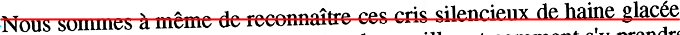
\includegraphics[width=500px, height=25px]{figures/exemple-ligne-decalee.png}}
\caption{Exemple d'erreur que fait l'EvaluateurPositionligne lorsque les lignes sont décalées}{Dans cette image, la ligne rouge représente le centroide vertical, qui est calculé pour être entre les y1 moyen et les y2 moyen de la ligne. Vu que la ligne est décalée, certaines lettres se trouvent à être plus haut que le centroïde vertical et sont alors considérées comme des appels}
\label{erreur-evaluateurpositionligne}
\end{figure*}
\label{tableau-evaluateurs}
\caption{Évaluateurs d'appels utilisés dans le prototype}
\end{table}
L'ensemble d'évaluateurs le plus simple qui soit a été utilisé dans un premier temps pour obtenir les valeurs sur lesquelles se baser pour optimiser la solution. Les combinaisons utilisées pour le prototype sont présentées à la page~\pageref{combinaisons-evaluateurs}.
\begin{table}
\begin{tabular}{| p{6cm} | p{2cm} | p{1.25cm} | p{6cm} |}
    \hline
    \rowcolor[gray]{0.9}
    Evaluateurs & Précision & Rappel & Observations et hypothèses \\
    EvaluateurAppelPositionLigne, EvaluateurAppelAlphaNum et EvaluateurAppelTaile (Seuil = 0.6)
    & $0.30$ & $0.28$ & 
    \begin{itemize}
        \item Les appels non numériques peuvent être enlevés (il y en a aucun dans le texte)
        \item Beaucoup d'erreurs dans les pages dont la numérisation est mal alignée. Peut-être dû au fait que l'algorithme ne tient pas compte de ce décalage en calculant les 
        \item Certaines erreurs sont dûes au fait que l'évaluateur trouve uniquement un appel (sans terme qui le porte).
        \end{itemize}  \\ \hline
        EvaluateurAppelPositionLigne,
        EvaluateurAppelNumerique et 
        EvaluateurAppelTaille (Seuil = 0.6)
    & $1.0$ & $0.37$ &
    \begin{itemize}
        \item Précision augmentée à 100\% depuis que seuls les chiffres sont considérés comme des appels.
        \item Tester l'evaluateur d'appel de régression linéaire.
    \end{itemize} \\
    \hline
        EvaluateurAppelPositionLigne (régression linéaire),
        EvaluateurAppelNumerique et
        EvaluateurAppelTaille (Seuil = 0.6)
    & $1.0$ & $0.37$ &
    \begin{itemize}
        \item Aucune amélioration depuis que la position par rapport à la ligne est calculée avec une droite de régression linéaire. 
        \item La majorité des erreurs sont dûes à un changement de notation de l'appel. 
    \end{itemize}
        \\ \hline
    EvaluateurAppelPositionLigne, EvaluateurAppelNumerique et EvaluateurAppelTaille pour la première partie. EvaluateurAppelDecalage, EvaluateurAppelNumerique et EvaluateurAppelTaille pour la deuxième partie &
    $0.78$ & $0.86$ &
    Baisse de la précision dûe au fait que les références à une page sur une ligne où il n'y a pas beaucoup de texte (ex: "p. 88") sont identifiés comme des appels puisque les chiffres sont plus haut que le caractère (donc décalés).
    \\ \hline
    \emph{idem.} & $0.82$ & $1.0$ &
    Amélioré le rappel en enlevant l'ÉvaluateurAppelTaille de la deuxième section. Amélioré la précision en ajoutant une règle qui agit au niveau du mot pour éliminer les cas où une référence à un numéro de page est interprété comme étant un appel.
    \\ \hline
\end{tabular}
\caption{Combinaisons d'évaluateurs d'appel utilisés dans le prototype}
\label{combinaisons-evaluateurs}
\end{table}

\subsubsection{Problèmes rencontrés et améliorations possibles}
Le problème principal a été dû à la qualité de la reconnaissance de caractères faite par tesseract. Bien que les résultats obtenus soient de manière générale satisfaisants, la reconnaissance des caractères d'appel s'est avérée très imprécise. En effet, dans la première partie, où les caractères d'appel étaient caractérisés par une plus petite taille et une position en appel, ces derniers ont la plupart du temps été confondus avec des caractères de ponctuation divers, par exemple l'apostrophe ou l'accent circonflexe.

Une configuration générique de tesseract a été utilisée pour faire la reconnaissance: les fichiers de langue française fournis avec la distribution \emph{Arch Linux}. Il serait possible d'améliorer la configuration de tesseract par une ou plusieurs des manières suivantes:
\begin{itemize}
    \item En entraînant tesseract pour la police particulière utilisée dans le document;
    \item En fournissant une liste de mots courants dans le document lors du lancement de tesseract. Cette liste de mots aide à préciser la numérisation en représentant plus fidèlement le modèle du texte numérisé;
    \item En fournissant une liste "DangAmbigs" comprenant les ambiguïtés couramment rencontrées dans le texte. Ce fichier contient les principaux de substitution dans une langue. Un exemple est fourni à la page~\pageref{figure-dangambigs}.
\end{itemize}

Entraîner tesseract en utilisant ces méthodes aurait pris du temps et aurait débordé du cadre du projet. Le fichier texte a plutôt été corrigé à la main, autant dans le fichier texte que dans le fichier \emph{boxfile}, lorsque c'était facile -- c'est-à-dire dans les cas autres que ceux où une lettre a été représentée par deux lettres (exemple h -> l n).

\begin{figure*}
\begin{lstlisting}
1	m	2	r n
2	r n	1	m
1	m	2	i n
2	i n	1	m
1	d	2	c l
...
...
\end{lstlisting}


\caption{Exemple de fichier DangAmbigs}{La première ligne indique que tesseract peut confondre un caractère (le m) pour deux caractères (r et n). La ligne suivante décrit le cas inverse, où deux caractères (r et n) sont confondus avec le m}
\label{figure-dangambigs}
\end{figure*}
Une autre limitation est due à l'implémentation de la solution. Les évaluateurs d'appel ont été implémentés pour évaluer une seule lettre à la fois et pour être initialisés à partir d'une ligne. Or, il serait préférable que ceux-ci puissent évaluer un mot au complet et être initialisés à partir du document au complet. Cette amélioration de conception aurait été utile pour certains évaluateurs, notamment celui détermine si un caractère est un appel à partir du ratio de la taille du caractère sur la taille moyenne des caractères d'une ligne. En l'entraînant à partir d'une seule ligne, il n'y a pas assez d'occurrences d'un même caractère de disponibles pour que ce soit une base de comparaison valide. La taille du caractère doit alors être comparée à la taille moyenne des autres caractères de la ligne nonobstant le contenu précis du caractère. Cela a comme effet que les caractères de ponctuation sont systématiquement perçus comme des appels, bien qu'en réalité ils ne le soient pas.



\subsubsection{Extraction des métadonnées}
La forme que prennent les citations dans le texte est déterminée selon une convention. Mais au-delà du fait que la convention invite l'auteur à fournir toutes les informations pertinentes qui pourraient aider le lecteur à retracer l'oeuvre citée, elle n'oblige à aucun formalisme. Ainsi, le format des références peut varier grandement. La figure~\ref{f4} montre les quelques premières citations de notre échantillon.

\fontsize{3.5mm}{4.5mm}\selectfont
\begin{table}
\begin{tabular}{| p{8cm} | p{8cm} | }
    \hline
    \rowcolor[gray]{0.9}
    Exemple & Format \\
    L'idéologie allemande, Paris, La Pléiade, 1982, p. 1085. & <TITRE>, <VILLE>, <COLLECTION>, <ANNÉE>, p. <PAGE>. \\
    \hline
    "Fini le règne des idéologies, place aux acteurs sociaux, Le Devoir, mercredi le 7 janvier 1987. & "<TITRE>, <PUBLICATION>, <DATE>. \\
    \hline
    \multicolumn{2}{|l|}{Note: le guillemet anglais manquant est dans le texte.} \\ 
    \hline
    Voir ici le texte de Alain Caillé & Voir <PUBLICATION> le texte de <AUTEUR> \\
    \hline
    Nicole Gagnon, La réforme scolaire au Québec, Université Laval, 1986 & <AUTEUR>, <TITRE>, <ÉDITEUR>, <ANNÉE> \\
    \hline
    Ou encore: "At last count, 50 percent of the American population believed an accused individual guilty until proven innocent; 50 percent didn't know which side the United States support in Nicaragua; 42 percent couldn't name an asian country "near the pacific ocean"; and 40 percent of the nation's High School seniors thought that Israel was an arab country". Lewis H. Lapham, Harper's Magazine, september 1987, p. 8. & <NOTE>, <AUTEUR>, <PUBLICATION>, <DATE>, <PAGE> \\
    \hline
    Les emplois en 1990: les options gagnantes, Ministère de l'Éducation, cité par Paul Bernard, "Imaginer le réel pour réaliser l'imaginaire", La sociologie et l'anthropologie au Québec, Cahiers de l'ACFAS, 1985, p. 112. & <TITRE-ORIGINAL>, <ÉDITEUR-ORIGINAL>, cité par <AUTEUR>, <TITRE-TEXTE>, <TITRE>, <ÉDITEUR>, <ANNÉE>, p. <PAGE>. \\
    \hline
    \multicolumn{2}{|l|}{Note: le guillemet anglais manquant est dans le texte.} \\ 
    \hline
\end{tabular}

\caption{Exemples de citations trouvées dans le texte}
\label{f4}
\end{table}
\fontsize{4.5mm}{6.5mm}\selectfont
Selon Afzal \emph{et coll.} \cite{afzal2009improving}, cette variation de la forme de la citation est surtout induite par des facteurs humains (les éditeurs ont leur propre style, les auteurs peuvent faire des erreurs dans le titre d'un texte cité, etc.) et est l'un des problèmes majeurs dans la conception d'outils d'extraction de métadonnées.

On peut remarquer dans les exemples ci-dessus que le formalisme des citations les situe à mi-chemin entre un langage formellement codifié et le langage naturel. Plutôt qu'un ensemble de règles formelles, il s'agit de conventions (suivies à un degré plus ou moins grand dépendant des disciplines) qui ont été élaborées par des humains afin d'échanger de l'information. Il n'existe pas, au final, d'ensemble fermé de règles permettant de reconnaître l'ensemble des citations possibles.

Cette avenue a tout de même été testée en tentant de créer un ensemble exhaustif d'expressions régulières. L'hypothèse portée par cette solution est que les expressions régulières peuvent être classées par ordre de restrictivité. Ainsi, la première à être testée est celle qui permet de récupérer le plus de champs (par exemple: Nom, Prénom, Titre, Maison d'édition, Collection, Ville, Année, pages) et la dernière à être testée est celle qui récupère le moins de champs (par exemple: Nom, Titre, Année). Ainsi, si l'une des expressions régulières de l'ensemble est en mesure de retourner de l'information, on peut prendre pour acquis qu'il m'aurait pas été possible d'obtenir plus d'information autrement.

Le problème qui se pose rapidement est celui du critère d'ordonnancement. Comment peut-on distinguer le format "<Auteur>, <titre>, <collection>, <annee>" du format "<Auteur>, <titre>, <editeur>, <annee>", ou encore du format "<titre>. <Auteur>, <editeur>"? Ces champs ne sont pas caractérisés par un format quelconque qu'il serait possible de reconnaître avec une expression régulière. Au regard d'une expression régulière, les différents champs sont équivalents puisque les expressions régulières sont incapables de saisir leur contenu sémantique.

Les différentes manières d'exprimer les citations sont infinies, mais l'ensemble de règles qui les évaluera sera toujours fini. En créant les règles, on se rend rapidement compte que celles-ci doivent toujours être adaptées aux spécificités du domaine. 

Le choix final a plutôt été d'utiliser une librairie implémentée en \emph{ruby} et distribuée sur le site \emph{github} en logiciel libre. Cette librairie, \emph{anystyle-parser}~\cite{anystyleparser}, implémente des \emph{Conditional Random Fields} pour étiqueter les parties d'une citation. Elle est distribuée avec un ensemble d'entraînement et est donc rapidement utilisables.

Anystyle-parser a de manière générale bien réussi à étiqueter les parties d'un ensemble de citations trouvées sur \emph{Google Scholar}. La plupart des erreurs étaient dans le type d'entrée BibTeX, en confondant \emph{inproceedings} avec \emph{incollection}, par exemple. Par contre, en utilisant \emph{anystyle-arser} tel que distribué, son utilisation dans le contexte de ce projet a été un échec étant donné qu'aucune citation n'a pu être étiquetée convenablement sauf dans un seul cas (celui de la citation de Nicole Gagnon présentée ci-haut).

Ce faible taux de réussite peut être attribué à plusieurs facteurs. Dans un premier cas, il faut noter que le modèle fourni avec anystyle-parser ainsi que tout l'ensemble d'entraînement ont été faits en anglais. Il est donc normal que, si entraîné en anglais, le logiciel éprouve des difficultés à généraliser en français.

Les problèmes de généralisation dus à la langue française se font sentir d'autant plus que les notes de bas de page présentes dans le document utilisé sont très souvent écrites en texte libre. Dans les publications du domaine des sciences naturelles, appliquées ou de l'ingénierie, la distinction entre une note de bas de page et une référence bibliographique est plus claire que dans les sciences humaines. En sciences humaines, la référence bibliographique est présentée dans une note de bas de page, mais on ne peut pas réduire une note de bas de page à une référence bibliographique. Il faut prendre pour acquis qu'il y aura du texte avant et après la référence bibliographique: il est donc nécessaire de pouvoir extraire la référence bibliographique de son contexte, ce qu'\emph{anystyle-parser} n'est pas conçu pour faire -- il arrive tant bien que mal à donner des résultats sensés en anglais, mais en français l'étiquetage semble être totalement arbitraire.
